\documentclass{beamer}

\usepackage{../Research}

\newcommand{\F}{\mathcal F}
\newcommand{\curly}[1]{\left\{ #1 \right\}}

\title{VC-density in model theoretic structures}
\author{Anton Bobkov}
\date{June 3, 2015}


\begin{document}

\maketitle

\begin{frame}
	Suppose we have an (infinite) collection of sets $\F$. \\
	We define the shatter function $\pi_\F \colon \N \arr \N$ of $\F$

	\begin{align*}
		\pi_\F(n) = \max \{ &\text {\# of atoms in boolean algebra generated by $\mathcal S$} \\
		            &\mid \mathcal S \subset \F \text{ with } |\mathcal S| = n\}
	\end{align*}
\end{frame}

\begin{frame}
	Example: Let $\F$ consist of all discs in the plane.
	\begin{figure}[p]
    \centering
    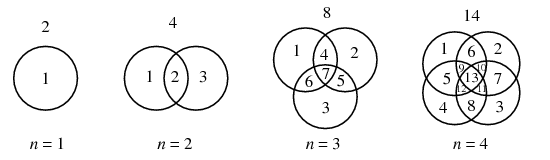
\includegraphics[scale=0.75]{circle.png}
	\end{figure}
	\begin{align*}
		\pi_\F(1) = 2 \ \ \  \pi_\F(2) = 4 \ \ \  \pi_\F(3) = 8  \ \ \ \pi_\F(4) = 14
	\end{align*}
	\begin{align*}
		\pi_\F(n) = n^2 - n + 2
	\end{align*}
\end{frame}

\begin{frame}
More examples: \\
	\begin{enumerate}
		\item Lines in the plane $\pi_\F(n) = n^2/2 + n/2 + 1$
		\item Disks in the plane	$\pi_\F(n) = n^2 - n + 2$
		\item Balls in $\R^3$  $\pi_\F(n) = n^3/3 - n^2 + 8n/3$
		\item Intervals in the line $\pi_\F(n) = 2n$
		\item Half-planes in the plane $\pi_\F(n) = n(n+1)/2 + 1$
		\item Finite subsets of $\N$ $\pi_\F(n) = 2^n$
		\item Convex polygons in the plane $\pi_\F(n) = 2^n$
	\end{enumerate}
\end{frame}

\begin{frame}
	\begin{Theorem} [Sauer-Shelah '72]
		The shatter function is either $2^n$ or bounded by a polynomial.
	\end{Theorem}
	\begin{Definition}
		Suppose the growth of the shatter function of $\F$ is polynomial.
		Let $\vc(\F)$ infimum of all positive reals $r$ such that
		\begin{align*}
			\pi_\F(n) = O(n^r)
		\end{align*}
		Call $\vc(\F)$ the vc-density of $\F$.
		If the shatter function grows exponentially, we let $\vc(\F) := \infty$.
	\end{Definition}
\end{frame}

\begin{frame}
	\frametitle{Applications}
	\begin{itemize}
		\item NIP theories
		\item VC-Theorem in probability (Vapnik-Chervonenkis '71)
		\item Computational learning theory (PAC learning)
		\item Computational geometry
		\item Functional analysis (Bourgain-Fremlin-Talagrand theory)
		\item Abstract topological dynamics (tame dynamical systems)
	\end{itemize}
\end{frame}

\begin{frame}
	\frametitle{History}
	\begin{itemize}
		\item Vapnik-Chervonenkis '71 - introduced VC-dimension
		\item NIP theories (Shelah '71, '90)
		\item vc-density (Aschenbrenner, Dolich, Haskell, Macpherson, Starchenko '13)
	\end{itemize}
\end{frame}

\begin{frame}
	\frametitle{Model Theory}
	Model Theory studies definable sets in first-order structures.
	\begin{align*}
		(\Q, 0, 1, +, \cdot, \leq)
	\end{align*}
	\begin{align*}
		\phi(x) = \exists y \ y \cdot y = x
	\end{align*}
	$\phi(\Q)$ defines the set of rationals that are a square.
\end{frame}

\begin{frame}
	\begin{align*}
		(\R, 0, 1, +, \cdot, \leq)
	\end{align*}
	\begin{align*}
		\phi(x) = \exists y \ y \cdot y = x
	\end{align*}
	$\phi(\R)$ defines the set $[0, \infty)$.
\end{frame}

\begin{frame}
	\begin{align*}
		(\R, 0, 1, +, \cdot, \leq)
	\end{align*}
	\begin{align*}
		\psi(x_1, x_2) = (x_1 \cdot x_1 + x_2 \cdot x_2 \leq 1.5) \wedge (x_1^2 \leq x_2)
	\end{align*}
	$\phi(\R^2)$ defines the set in $\R^2$ that is an intersection of a disc with an inside of a parabola.
\end{frame}

\begin{frame}
	We work with families of uniformly definable sets.
	Fix a formula $\phi(x_1 \ldots x_m, y_1, \ldots y_n) = \phi(\vec x, \vec y)$.
	Plug in elements from $M$ for $y$ variables to get a family of definable sets in $M^m$.
	\begin{align*}
		\F^M_\phi = \curly{\phi(M^m, a_1, \ldots a_n) \mid a_1, \ldots a_n \in M}
	\end{align*}
	Define $\vc^M(\phi)$ to be the vc-density of the family $\F^M_\phi$ \\
\end{frame}

\begin{frame}
	\begin{align*}
		\phi(x_1, x_2, y_1, y_2, y_3) = (x_1 - y_1)^2 + (x_2 - y_2)^2 \leq y_3^2
	\end{align*}
	In structure $(\R, 0, 1 +, \cdot, \leq)$ given $a,b,r \in \R$ the formula $\phi(x_1, x_2, a, b, r)$ defines a disk in $\R^2$ with radius $r$ with center $(a,b)$.
	Thus $\F^\R_\phi$ is a collection of all disks in $\R^2$.
\end{frame}

\begin{frame}
	Shelah ('78) classified number of isomorphism classes for structures elementarily equivalent to structure $M$.
	One of the important classes is NIP structures.
	Structure $M$ is said to be NIP if all uniformly definable families in it have finite $\vc$-density.
	\begin{itemize}
		\item $(\C, 0, 1, +, \cdot)$ is NIP
		\item $(\R, 0, 1, +, \cdot, \leq)$ is NIP
		\item $(\Q_p, 0, 1, +, \cdot, \mid)$ is NIP
		\item Random graph $(V, R)$ is not NIP
		\item $(\Q, 0, 1, +, \cdot)$ is not NIP.
	\end{itemize}
\end{frame}

\begin{frame}
	Given an NIP structure $M$ we define a vc-function of $n$ to be the largest $\vc$-density achieved by families of uniformly definable sets in $M^n$.
	\begin{align*}
		\vc^M(n) = max \curly{ \vc^M(\phi) \mid \phi(\vec x, \vec y) \text{ with } |\vec x| = n}
	\end{align*}
	Easy to show $\vc^M(n) \geq n \vc^M(1) \geq n$ \\

	Open Question: If $M$ is NIP, is it possible for $\vc^M(\phi)$ to be irrational?
	Open Question: Is $\vc^M(n) = n \vc^M(1)$? If not, is there a linear relationship? If $\vc(1) < \infty$ do we have $\vc(2) < \infty$?
\end{frame}

\begin{frame}
	Examples
	\begin{itemize}
		\item $(\R, 0, 1, +, \cdot, \leq)$ has $\vc(n) = n$ (true for o-minimal structures)
		\item $(\C, 0, 1, +, \cdot)$ has $\vc(n) = n$
		\item $(\Q_p, 0, 1, +, \cdot)$ has $\vc(n) \leq 2n - 1$
	\end{itemize}
\end{frame}

\begin{frame}
	\frametitle{vc-density in trees}
	Consider structure $(T, \leq)$ where elements of $T$ are vertices of a rooted tree and we say that $a \leq b$ if $a$ is below $b$ in the tree.
	\begin{itemize}
		\item Trees are NIP (Parigot '82)
		\item Trees are dp-minimal (Simon '11)
		\item Trees have $vc(n) = n$ (B. '13)
	\end{itemize}
\end{frame}

\begin{frame}
	\frametitle{proof background}
	$\tp(a)$, a type of an element $a$ is a set of all the formulas that that are true about $a$.\\
	Parigot's observation: there is a natural way to split a tree into parts $A, B$ such that for $a \in A$ and $b \in B$ we have
	\begin{align*}
		\tp(a), \tp(b) \vdash \tp(ab)
	\end{align*}
	This allows us to decompose complex types into simple parts, which we can use to compute $\vc$-density.
\end{frame}

\begin{frame}
	\frametitle{Shelah-Spencer graphs}
	Let $\alpha$ irrational $\in (0,1)$.
	Consider a random graph on $n$ vertices where the probability of the given two vertices having an edge is $n^{-\alpha}$.
	Shelah-Spencer graph is a limit of such graphs for $\alpha$ irrational in $(0,1)$.
	We view it in a language with a single binary relation.
	\begin{itemize}
		\item Shelah-Spencer graphs can be axiomatized (Shelah-Spencer '88)
		\item Shelah-Spencer graphs are stable (Baldwin-Shi '96, Baldwin-Shelah '97 )
	\end{itemize}
\end{frame}

\begin{frame}
	\frametitle{Background}
\begin{Definition}
	\begin{itemize}
		\item To a finite graph $A$ assign a dimension $\delta(A) = |V| - \alpha |E|$.
		\item $B/A$ is called a positive extension if quantity $\delta(B/A) = |V_B/V_A| - \alpha |E_B/E_A|$ is positive.
		\item $B/A$ is called minimal if its dimension is negative, but every subextension is positive.
		\item $(A_0, \ldots A_n)$ is a minimal chain if each $A_{i + 1}/A_i$ is minimal.
	\end{itemize}
\end{Definition}
	For $B/A$ chain-minimal define
	\begin{align*}
		\phi_{A,B}(\vec x) = \exists \vec y \text { such that $\vec y/\vec x$ is isomorphic to $B/A$}
	\end{align*}
	\begin{Theorem} [quantifier elimination]
		In Shelah-Spencer graph every definable set can be defined by a boolean combination of formulas $\phi_{A_i, B_i(\vec x, \vec y)}$.
	\end{Theorem}
\end{frame}

\begin{frame}
	\frametitle{vc-density in Shelah-Spencer graphs}
	
	\begin{itemize}
		\item $\vc(1) = \infty$, so vc-function is not well-behaved for this structure.
		\item For a formula $\phi(\vec x, \vec y)$ we can define $\epsilon_L, \epsilon_U$ (with a simple dependence on $\delta(B_i/A_i)$) such that
			\begin{align*}
				\epsilon_L |\vec x| \leq \vc(\phi) \leq \epsilon_U |\vec x|
			\end{align*}
	\end{itemize}
\end{frame}

\begin{frame}
	\frametitle{Future work}
	\begin{itemize}
		\item $(\Q_p, 0, 1, +, \cdot, \mid)$
		\item Other partial orderings, lattices
		\item Other graph structures, in particular flat graphs
	\end{itemize}
\end{frame}

\end{document}


\begin{frame}
	To a finite graph $A$ assign a dimension $\delta(A) = |V| - \alpha |E|$. $B/A$ is an extension. $\delta(B/A)$ is $\delta(A) = |V_B/V_A| - \alpha |E_B/E_A|$. $B/A$ is called minimal if its dimension is negative, but every subextension is positive. $(A_0, \ldots A_n)$ is a minimal chain if each $A_{i + 1}/A_i$ is minimal.
	Any 
\end{frame}

